\subsubsection{Budget du projet}
Le budget total du projet s’élevait à \textbf{~2 700 €}, répartis comme suit :

\begin{figure}[h!]
    \centering
    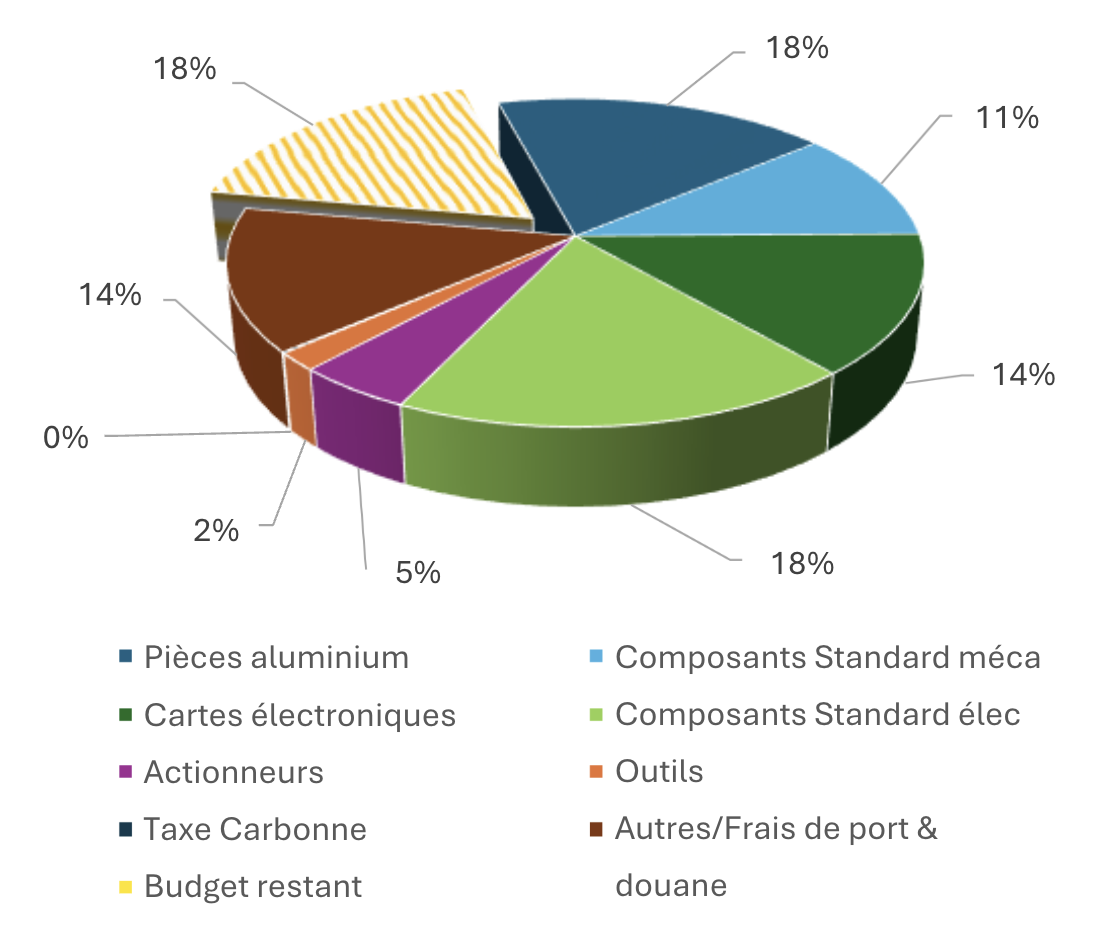
\includegraphics[width=\textwidth]{figures/graph_budget.png}
    \caption{Répartition du budget du projet SP-02}
    \label{fig:budget_projet}
\end{figure}


\subsubsubsection{Optimisations futures}
\begin{itemize}
    \item \textbf{Commandes groupées} : Organiser davantage de commandes groupées pour limiter les frais de ports/douane...
    \item \textbf{Partenariats} : Collaborer davantage avec des entreprises locales et/ou spécialisées pour obtenir des matériaux à moindre coût.
    \item \textbf{Prévision des imprévus} : Allouer 15\% du budget à une marge pour les aléas des frais de douanes plus importants que prévus malgré leur prévision, et une marge d'erreur pour la refabrication de composants dûs à des modifications de dernière minute.
\end{itemize}
